\documentclass[twocolumn,aps,showpacs,superscriptaddress,prl]{revtex4}

\usepackage{amsmath,amssymb,graphicx}
\usepackage{bm}
\usepackage{algorithmic}
\usepackage{enumerate}
\usepackage{color}
\usepackage{stmaryrd}
\usepackage{times}
\def\comment#1{{\bf\color{red}#1}}
\def\cm#1{{\bf\color{red}#1}}


\newcommand{\W}{W} 
\newcommand{\pbc}{\pi}
\newcommand{\abc}{\overline{\pi}}
\newcommand{\lav}{\bm{\langle}}
\newcommand{\rav}{\bm{\rangle}}

\newcommand{\cJ}{{\cal J}}
\newcommand{\D}{\Gamma_{\ell}}
\newcommand{\PJ}{P_{\cal J}(q)}
\newcommand{\PD}{P(q)}

\newcommand{\T}{S}
\newcommand{\ratio}{\Gamma_s}


\begin{document}

\title{Calculation of Boundary Condition in the Migdal-Kadanoff Spin Glass and Size Chaos}


\author{Jeff Gertler}
\email{jgertler@physics.umass.edu}
\affiliation{Department of Physics, University of Massachusetts,
Amherst, Massachusetts 01003 USA}


\author{Jonathan Machta}
\email{machta@physics.umass.edu}
\affiliation{Department of Physics, University of Massachusetts,
Amherst, Massachusetts 01003 USA}
\affiliation{Santa Fe Institute, 1399 Hyde Park Road, Santa Fe, New Mexico
87501, USA}

\begin{abstract}

Abstract here

\end{abstract}

\pacs{75.50.Lk, 75.40.Mg, 05.50.+q, 64.60.-i}
\maketitle



\paragraph*{Boundary Condition Calculation} ---

The Migdal-Kadanoff Renormalization Group offers a method of investigating large spin glass systems within realistic computation times. It takes advantage of a hierarchical structure which can be tailored for any dimension. For this paper we use the necklace structure with d=3 (cite Machta 1993). This geometry has be shown to provide results comparable to the euclidean d=3 spin glass (gonna need that citation). The renormalization group is generated by the comparison of partition functions which yields formulas for combining bonds in parallel and series.



% Parallel bonds
\begin{equation}
K' = K_1 + K_2
\label{eq:par}
\end{equation}

% Series bonds
\begin{equation}
K' = \frac{1}{2}\ln \Big(\frac{\cosh(K_1+K_2)}{\cosh(K_1-K_2)} \Big)
\label{eq:ser}
\end{equation}

% MKRG
\begin{equation}
K' = \frac{1}{2}\ln \Big(\frac{\cosh(K_1+K_2+K_3+K_4+K_5+K_6+K_7+K_8)}{\cosh(K_1+K_2+K_3+K_4-K_5-K_6-K_7-K_8)} \Big)
\label{eq:mkrg}
\end{equation}





\begin{figure}[htb]
\begin{center}
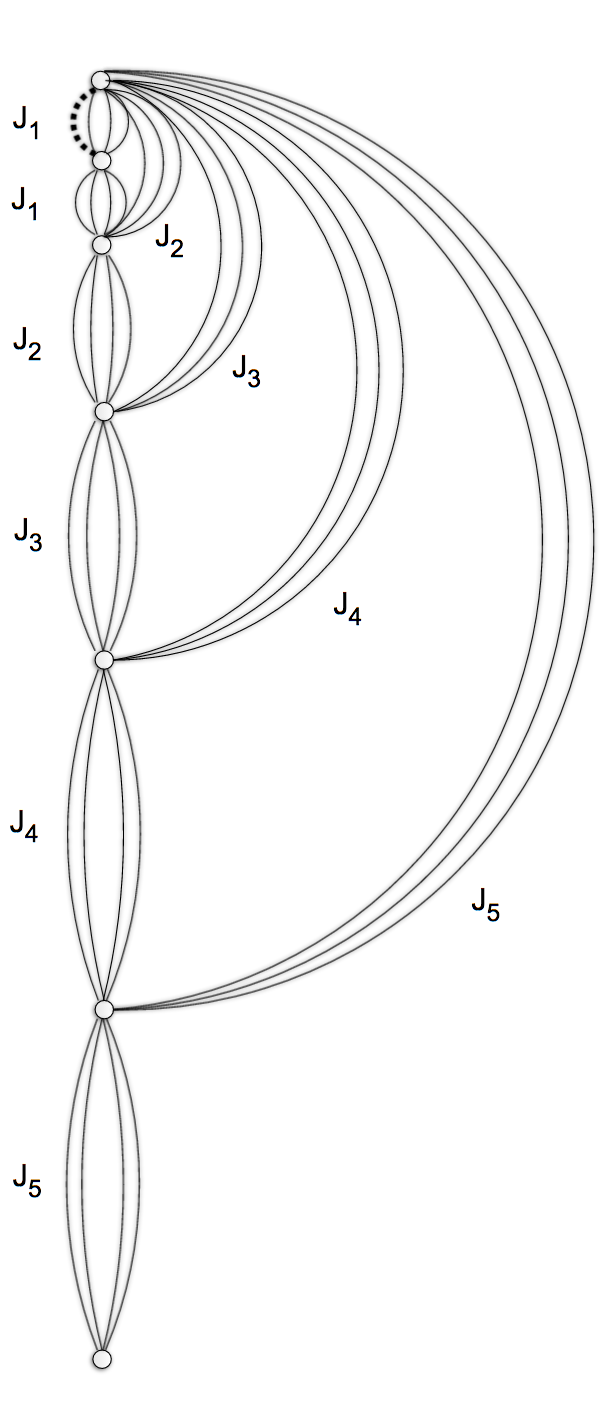
\includegraphics[width=0.5\columnwidth]{full_diag.png}
\caption{
Full Migdal-Kadanoff latice.
}
\label{Pq3}
\end{center}
\end{figure}

\begin{figure}[htb]
\begin{center}
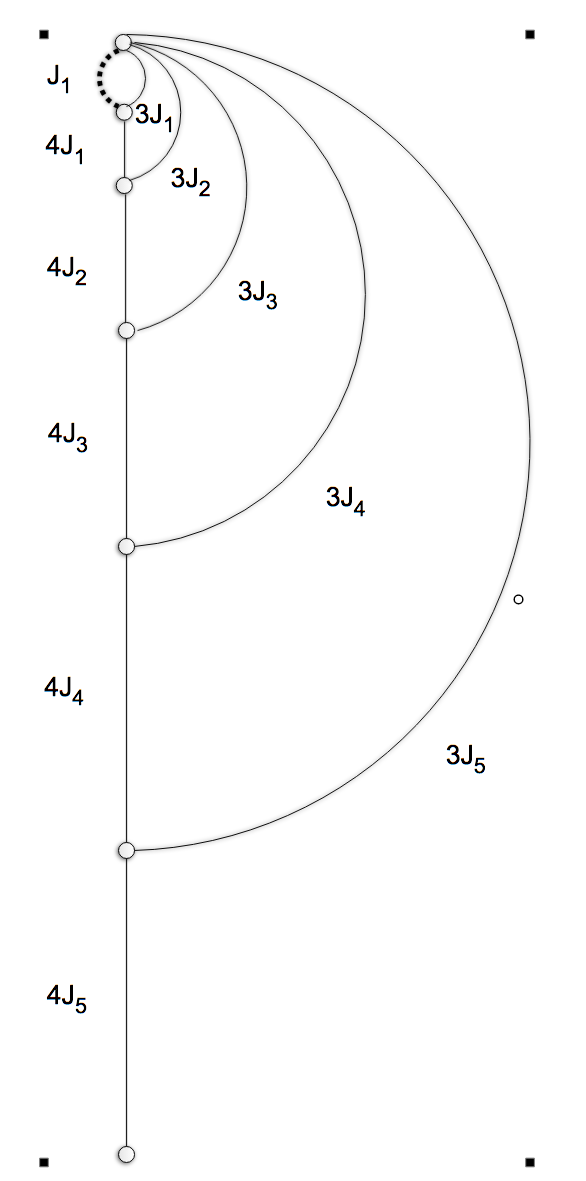
\includegraphics[width=0.5\columnwidth]{reduced_diag.png}
\caption{
Reduced Migdal-Kadanoff through parallel equation.
}
\label{Pq3}
\end{center}
\end{figure}

% BC Calculation
\begin{equation}
\begin{split}
K_{BC} = 3K_1 + (4K_1:(3K_2 + 4K_2:(3K_3 \\
+ 4K_3:(3K_4 + 4K_4:(3K_5+ ...)))))
\end{split}
\label{eq:bc}
\end{equation}


\paragraph*{Size Chaos} ---

% Correlation function
\begin{equation}
F(n) = | \tanh(K_n) - \tanh(K_{\inf}) |
\label{eq:cor}
\end{equation}



\begin{acknowledgments}

Some stuff here.

\end{acknowledgments}

\bibliographystyle{apsrevtitle}
\bibliography{refs}

\end{document}
